\begin{itemize}
    \item The Bayes classifier directly uses the Bayes theorem to predict the class for a new test instance, x. It estimates the posterior probability $P (c_i|x)$ for each class $c_i$ , and chooses the class that has the largest probability. The predicted class for x is given as
    \[ y = \operatorname*{argmax}_{c_i} P (c_i|x)\]
    \[ P (c_i|x) = \frac{P(x|c_i)P(c_i)}{P(x)}\]
    or for ease we can discard P(x).
    \item Estimate Prior Probability: $P(c_i) = \frac{n_i}{n}$
    \item Estimate probability of observing x from any of the k classes: $$P(x) = \sum_{j=1}^k{P(x|c_j)P(j)}$$
    \item Estimate Likelihood of Numeric attribute:
\begin{figure}[H]
\centerline{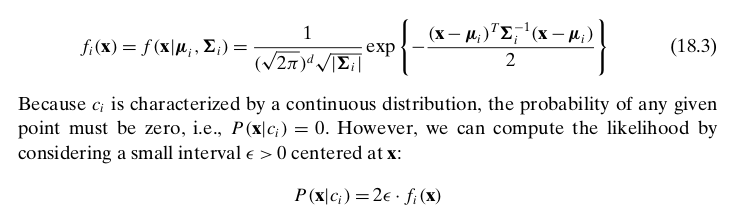
\includegraphics[width=1.3\textwidth]{Figures/bayes1.png}}
\end{figure}
    \item Estimate Likelihood of Categorical attribute:
\begin{figure}[H]
\centerline{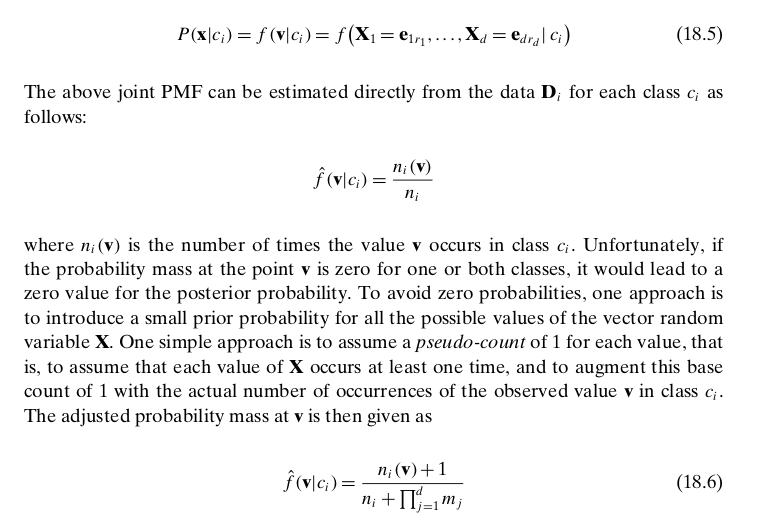
\includegraphics[width=1.1\textwidth]{Figures/bayes2.png}}
\end{figure}  
\begin{figure}[H]
\centerline{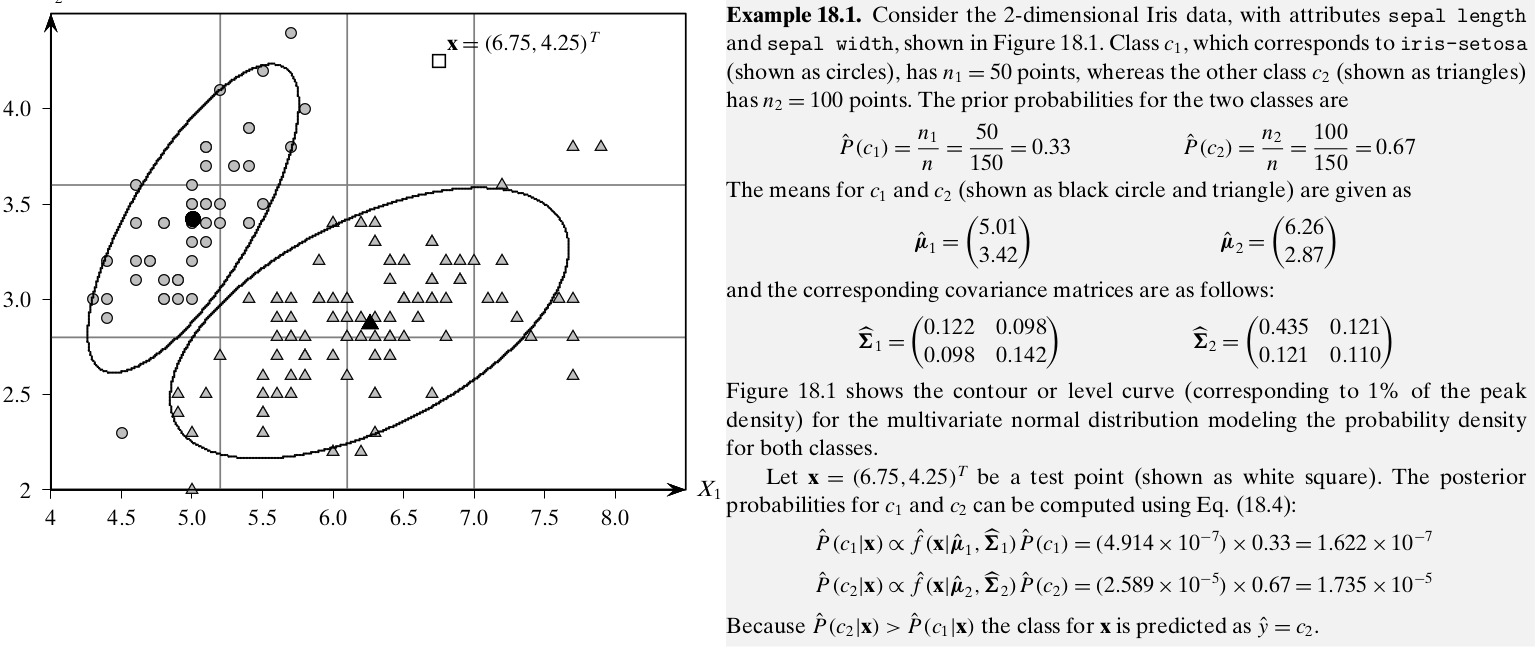
\includegraphics[width=1.3\textwidth]{Figures/bayes_ex}}
\end{figure}
    \item Classes are parameterized with mean vector and covariance matrix.This might not hold true for all cases.Too many parameters to be estimated. (For numeric attributes, $O(d^2)$ covariances).  Use Naive !
\begin{figure}[H]
\centerline{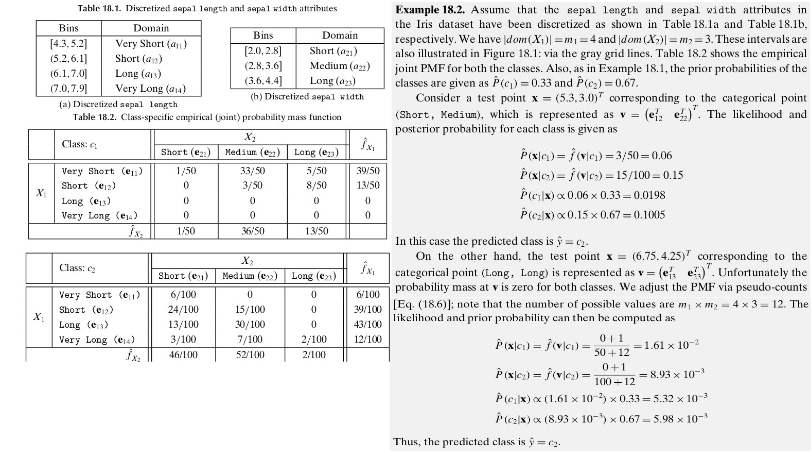
\includegraphics[width=1.2\textwidth]{Figures/bayes3}}
\end{figure}
    
\end{itemize}